\documentclass{article}
\usepackage[utf8]{inputenc}
\usepackage{fancyhdr}
\usepackage{graphicx}
\usepackage{geometry}

% ---- Commands ------- %
\newcommand{\documentNumber}[1]{
    \LARGE  \textbf{ PUSS2142{#1} } \\
    \medskip
}
\newcommand{\documentVersion}[1]{
    v. {0.2}

    \medskip
}
\newcommand{\documentTitle}[1]{
    \centerline{\rule{13cm}{0.4pt}}
    \bigskip \bigskip
    \LARGE {#1} \\
    \bigskip \bigskip
    \centerline{\rule{13cm}{0.4pt}}
}
\newcommand{\documentGroup}[1]{
    \bigskip \bigskip
    \LARGE Group {#1} \\
    \bigskip
}
\newcommand{\documentResponsible}[1]{
    \LARGE Responsible: {#1} \\
    \medskip
}
\newcommand{\documentAuthors}[1]{
    \LARGE Authors: {#1} \\
    \medskip    
}
\newcommand{\documentDate}[1]{
    \date {#1} 
}

\graphicspath{{./images/}} % Defines a path to file images
\renewcommand{\arraystretch}{1.7}  % Vertical padding for tables


% --- Header & Footer ---- %
\pagestyle{fancy}
\lhead{\leftmark}
\rhead{}
\rfoot{\thepage}
\cfoot{}
\lfoot{}


% ------------------------------------------------ #

% ----- FILL THIS ----- %
\title {
    % Must be 2 digits
    \documentNumber {01}    
    
    \documentVersion {0.1}
    
    % Full name - SHORTNAME
    \documentTitle {SRS - Software Requirements Specification}
    \documentGroup {2}
    
    % Options: - Project management Group
    %          - System architecture Group
    %          - Developer Group
    %          - Test Group
    \documentResponsible {System Group}
    \documentAuthors {System Group, UG}
    
    % Format: YYYY-MM-DD
    \documentDate {2021-02-02}
}

\begin{document}
\addtocontents{toc}{\protect\setcounter{tocdepth}{2}}
\maketitle
\thispagestyle{empty}

\newpage

\tableofcontents

\newpage



\section{Introduction}

This document presents requirements for the (Sätt in namn). (Sätt in namn) is a system which purpose and main functionality is to administer time reporting with web-usage capabilities. 


\section{Reference documents}

\begin{enumerate}
  \item Software Requirements Specification: BaseBlockSystem, v. 1.0, Doc. number: PUSS12002
  \item The requirements on the usability of the system applies to this document and are therefore implemented in “System-namn”, following requirements are implemented; 6.1.1, 6.1.2, 6.1.3, 6.1.4, 6.1.6, 6.1.7, 6.1.8, 6.1.9, 6.2.2, 7.1.1, 7.2.1
\end{enumerate}

\section{Background and goals}
\subsection{Main goals}

The goal is to develop and distribute a web-based system where the user can report time and administrate the system according to their roles.

\subsection{Actors and their objectives}
The system can be used and administrated by following actors;

\begin{itemize}
  \item \textbf{User:} The user has the authority to log in to the system to report and  change past reported time as well as review their reported times. The user also inherits roles as either "PG", "SG", "UG", and "TG".
  \item \textbf{Project Leader:}
  The project leaders main objective is to administer groups within the project, this implies that the project leader has the authority to add and remove as well as assign users from/to designated roles.
   \item \textbf{Administrator:} The administrator has the authority to add and remove users from the system along with creating and removing project groups. The admin is the only role that can assign the role “Project leader” to a user. The main goal of this role is to be able to administrate creation and removal of users.
\end{itemize}




\section{Terminology}



\section{Context diagram}
\begin{figure}[placement specifier]
\centering
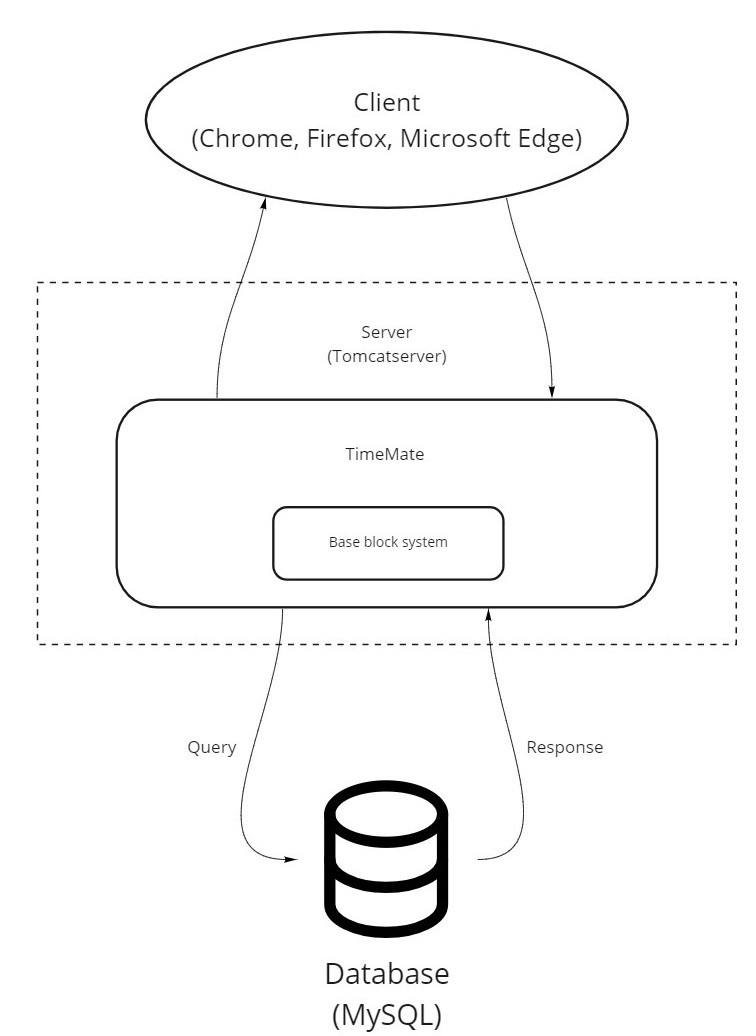
\includegraphics[width=0.5\textwidth]{Flowchart_6.jpg}
\caption{Context diagram}
\end{figure}

\section{Functional requirements}
\subsection{Login and logout}


\subsubsection{Requirement}
If the user has forgotten their password, they should be able to get a newly generated password from the server by email.

\subsubsection{Requirement}
New users should be assigned passwords generated by the server according to the password ruleset and recieve it by email.



\begin{figure}[placement specifier]
\centering
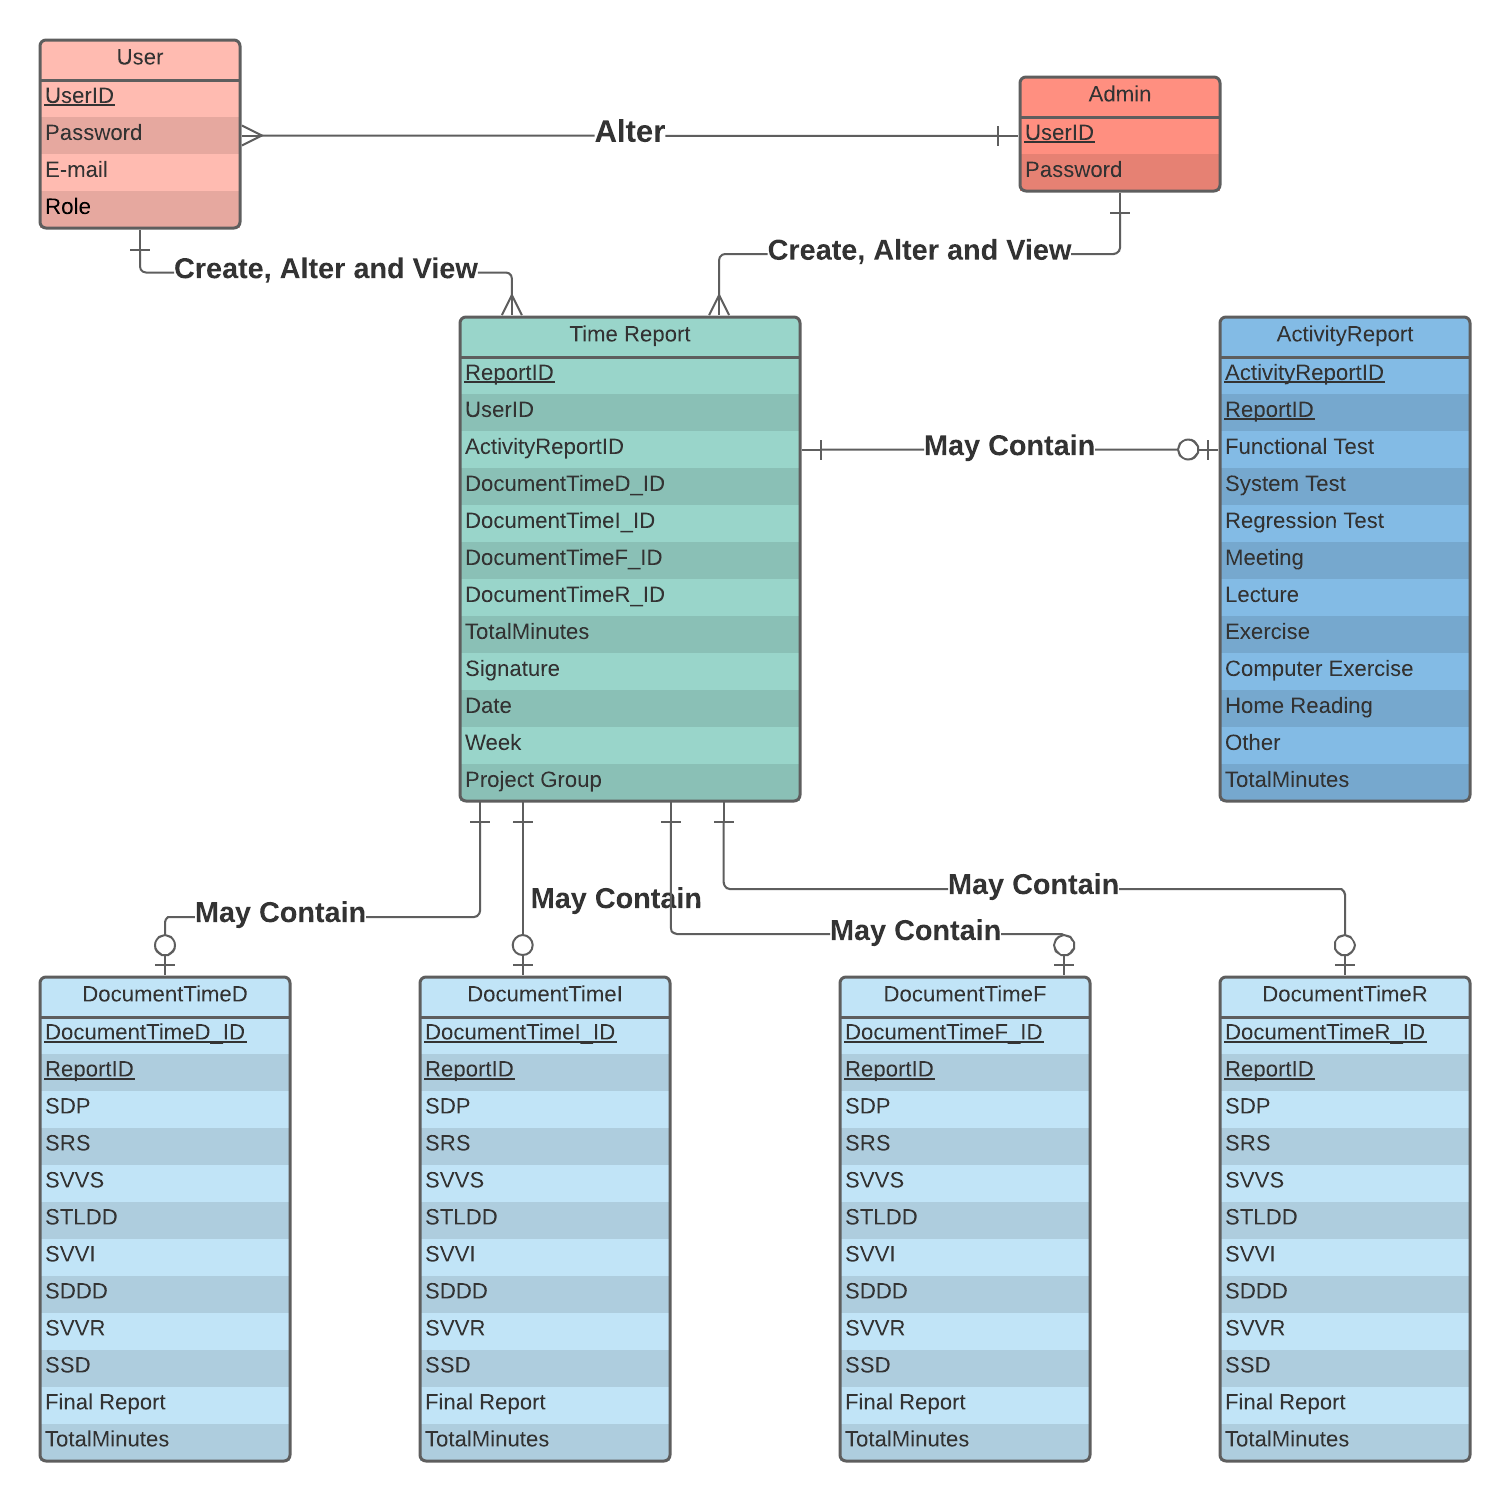
\includegraphics[width=0.5\textwidth]{PUSPERdiagram.png}
\caption{ER-diagram}
\end{figure}





\subsection{Data}
\subsubsection{Requirement}
A password should consist of at least one character of each type. [a-z][A-Z][1-9] with a minimum of 8 characters.

\subsection{User}
\subsubsection{Requirement}
A user can create and submit a time report to the project group which they are assigned to.
\subsubsection{Requirement}
The following scenario should be supported by the system.

\textbf{Scenario:} The user wants to submit a time report

\textbf{Prerequisites} The user is logged in to the system

\begin{enumerate}


\item The user navigates to the page “Time Report”. 
\item The user is presented with an overview of their previously reported time. 
\item The user presses the button “Create New Time Report”
\item The user fills in the blank textboxes with the time in minutes they have spent on the different activities.
\item The user presses the button for “Submit”.
\item The user is presented with a popup window confirming that the changes have been made.
\item An updated view of the page is displayed.
\end{enumerate}

\subsubsection{Requirement}
A user should be able to see a summarized view of previous reported time.

\subsubsection{Requirement}
The following scenario should be supported by the system.

\textbf{Scenario:} The user wants to see a summary of their reported time.

\textbf{Prerequisites} The user is logged in to the system
\begin{enumerate}


\item The user navigates to the page “Time report”.
\item A page is displayed which includes the option to report time, edit old time reports but also review a summarized view of their previously logged time. 
\end{enumerate}

\subsubsection{Requirement}
A user should be able to change their time report after it has been submitted to the system.

\subsubsection{Requirement}
The following scenario should be supported by the system.

\textbf{Scenario:} A user wants to change previously reported time.

\textbf{Prerequisites} The user is logged in to the system

\begin{enumerate}

\item The user navigates to the page “Time report”.
\item The user is presented with an overview of their previously reported time. 
\item The user presses the button “Edit time report”
\item The user chooses a time report.
\item The user is presented with a new page which includes the previously reported time table and a button for “Delete”. 
\item The user adds/fills in the new time or chooses to delete the report.
\item The user clicks on the button “Submit Change”.
\item The user is presented with a popup window confirming that the changes have been made.  
\item An updated view of the page is displayed.

\end{enumerate}


\subsubsection{Requirement}
Users should be able to change their password on the “My profile” page.
\subsubsection{Requirement}
Users changing their passwords should not be able to set their new password to be the same as their current password.

\subsubsection{Requirement}
The following scenario should be supported by the system.

\textbf{Scenario:} A user wants to change their password.

\textbf{Prerequisites} The user is logged in to the system

\begin{enumerate}
    \item The user clicks on the “Change Password” button in the menu.
    \item The user is presented with a page which includes three relevant textboxes.
    \item The user fills in the first textbox with their current password.
    \item The user fills in the second textbox with their new password.
    \item The user repeats their new password in the third textbox.
    \item The user clicks the button “Change Password”.
    \item The user's password is changed in the system.
    \item The user is presented with a popup window confirming that the changes has been made.
\end{enumerate}



\subsubsection{Requirement}
The following scenario should be supported by the system.

\textbf{Scenario:} A user wants to change their password with invalid entry.

\textbf{Prerequisites} The user is logged in to the system

\begin{enumerate}
    \item The user clicks on the “Change Password” button in the menu.
    \item The user is presented with a page which includes three relevant textboxes.
    \item The user fills in the first textbox with their current password.
    \item The user fills in the second textbox with their new password which does not meet requirement 6.2.1.
    \item The user repeats their new password in the third textbox.
    \item The user clicks the button “Change Password”.
    \item The user's password is not changed and a popup window with an error message is displayed.
    \item The user is sent back to stage 3.
\end{enumerate}

\subsubsection{Requirement}
Users should not be able to edit signed time-reports.

\subsection{Project Leader}
\subsubsection{Requirement}
The following scenario should be supported by the system.

\textbf{Scenario:} The project leader tries to acquire a summary of reported time.

\textbf{Prerequisites:} Time to be summarized exists, user has the role "Project leader" and the user is on the "Time Reporting" page.

\begin{enumerate}
    \item The project leader clicks on the administration page 
    \item The project leader clicks on the “SHOW SIGNED REPORTS” button.
    \item A list with user’s name and the total reported time will be displayed,
    \item The project leader clicks on a user name and it displays the user’s time reports.
\end{enumerate}

\subsubsection{Requirement}
The project leader can create and submit a time report.

\subsubsection{Requirement}
Project leader is able to view all project members and their individual roles.


\subsubsection{Requirement}
The project leader can change a project members role except themselves and other project leaders.

\subsubsection{Requirement}
Project leaders should be able to sign time-reports, making them uneditable.

\subsubsection{Requirement}
The following scenario should be supported by the system.

\textbf{Scenario:} Project leader tries to sign a weekly report

\textbf{Prerequisites:} User has the role ”Project leader”, weekly reports exists, and the project leader has clicked on the “Sign Time Reports” button.

\begin{enumerate}
    \item A list of all the unsigned weekly reports is shown to the project leader.
    \item The project leader can sign the reports by clicking on the corresponding checkbox.
    \item The project leader confirms their selection by pressing on the “Confirm” button
    \item The system sends the changes to the server.
    \item The system returns an updated list of unsigned reports, or an empty list if none exists
\end{enumerate}

\subsubsection{Requirement}
The following scenario should be supported by the system.

\textbf{Scenario:} Project leader tries to assign roles to members.

\textbf{Prerequisites:} User has the role “Project leader”, members exists and the user is on the “User Management“ page.

\begin{enumerate}
    \item The project leader can change members' roles by clicking on the corresponding radio button.
    \item Project leader confirms changes made by pressing “Confirm”.
    \item The system sends the changes to the server.
    
\end{enumerate}


\subsection{Administrator}

\subsubsection{Requirement}
All users in the database should be shown as a list on the “Administration” page.

\subsubsection{Requirement}
The administrator should be able to add and remove users.

\subsubsection{Requirement}
All requirements and scenario listed for "Users" and "Project Leaders" also apply to the administrator.

\subsubsection{Requirement}
The following scenario should be supported by the system.

\textbf{Scenario:} The administrator tries to add a user.

\textbf{Prerequisites:} The administrator is on the “Administration” page

\begin{enumerate}
    \item Administrator clicks on the button to add a user.
    \item Administrator inputs the name of the user.
    \item The inputs are sent to the server which adds it to the database and generates a password.
    \item The system creates a new entry in the user list and inserts the inputted name.
    \item The server returns the password to the corresponding field in the user list.
    \item The user clicks the button “Change Password”.
    \item The updated user list is shown to the administrator.
\end{enumerate}

\subsubsection{Requirement}
The following scenario should be supported by the system.

\textbf{Scenario:} The Administrator tries to add a user with the same name.

\textbf{Prerequisites:} The administrator is on the “Administration” page

\begin{enumerate}
    \item Administrator clicks on the button to add a user.
    \item Administrator inputs the name of the user.
    \item The inputs are sent to the server, which notices that the name already exists in the database.
    \item The server does not accept the inputted name.
    \item Administrator is told that the user already exists with a message.
\end{enumerate}

\subsubsection{Requirement}
The following scenario should be supported by the system.

\textbf{Scenario:} The administrator tries to remove a user.

\textbf{Prerequisites:} The administrator is on the “Administration” page

\begin{enumerate}
    \item Administrator clicks on the button to remove the user.
    \item Administrator must confirm the removal by typing in the user’s name and click on the “confirm” button.
    \item The information is sent to the server.
    \item The user is removed from the database.
    \item The page is updated with the new user list, with a message confirming the change.
\end{enumerate}


\subsubsection{Requirement}
The following scenario should be supported by the system.

\textbf{Scenario:} The administrator tries to acquire a summary of reported time.
\textbf{Prerequisites:} Time to be summarized exists.

\begin{enumerate}
    \item Administrator clicks on the administration page 
    \item Administrator clicks on the “SHOW SIGNED REPORTS” button.
    \item A list with the names of all the users and their total reported time will be displayed,
    \item Administrator clicks on a user name and it displays the user’s time reports.
\end{enumerate}

\subsubsection{Requirement}
The following scenario should be supported by the system.

\textbf{Scenario:} The administrator tries to assign a role to a user.

\textbf{Prerequisites:} The administrator is on the administration page.

\begin{enumerate}
    \item Administrator clicks on “view”.
    \item A list with all users and their roles is displayed.
    \item Administrator clicks on the role-alternative.
    \item Administrator can change the role of the user by clicking on a new role and confirming it.
    \item The information is saved and sent to the server
    \item The database is updated with the changes.
\end{enumerate}

\section{Design requirements}

\subsubsection{Requirement}
The main font should be web safe and belong to one of the following font
familes: Serif or Sans-serif.
\subsubsection{Requirement}
The main text should have a font size of 16 pixels (2 pixels). All main
text should be of the same size.
Textfields and textfield captions should have a font size of at least 16
pixels.
\subsubsection{Requirement}
The color scheme should consist of three primary colors. These should, if
possible, follow the 60/30/10 design rule. Secondary colors are permitted
only when dealing with less important information.
The background should consist of a lighter color and the main text should
consist of a darker shade.
\subsubsection{Requirement}
The content of the web page should be centered in the browser window.
The content should keep its centered position when the window is ex-
tended.
\subsubsection{Requirement}
A fixed navigation/menu bar shall be placed horizontally at the very top
of the page.
\subsubsection{Requirement}
Selections Main-page, Administration, User Management, Time Reporting
and My profile should be included in the menu bar. Other menu selections
should be categorized as subheadings belonging to one of the primary
menu choices and should not be visible or clickable by default.
The administrators should have an additional menu selection called Ad-
ministration.
\subsubsection{Requirement}
When a menu selection containing at least one subheading is selected a
vertical menu bar containing its subheadings should be revealed.
A downward pointing arrowhead, should be placed next all menu selections containing at least one subheading. 
When a menu selection containing one or more subheadings is selected, the arrowhead should point
upwards.

\subsubsection{Requirement}
The system logo and/or the system name shall be placed on the far left
of the menu bar.

\section{Project requirements}
\subsection{Development environment}
\subsubsection{Requirement}
The back end for the system should use Java JDK 11 as development environment.

\subsubsection{Requirement}
The front end for the system should use Bootstrap v.4.5.3.

\subsubsection{Requirement}
The database should be developed in MySQL.

\subsubsection{Requirement}
Error messages should be in the following format: ”Error code – Reason”.

\end{document}
